\documentclass{article}

\usepackage{tikz} 
\usetikzlibrary{automata, positioning, arrows} 

\usepackage{amsmath}
\usepackage{amsthm}
\usepackage{amsfonts}
\usepackage{amsmath}
\usepackage{amssymb}
\usepackage{fullpage}
\usepackage{color}
\usepackage{parskip}
\usepackage{graphicx}
\usepackage{hyperref}
  \hypersetup{
    colorlinks = true,
    urlcolor = blue,       % color of external links using \href
    linkcolor= blue,       % color of internal links 
    citecolor= blue,       % color of links to bibliography
    filecolor= blue,        % color of file links
    }
    
\usepackage{listings}

\definecolor{dkgreen}{rgb}{0,0.6,0}
\definecolor{gray}{rgb}{0.5,0.5,0.5}
\definecolor{mauve}{rgb}{0.58,0,0.82}

\lstset{frame=tb,
  language=haskell,
  aboveskip=3mm,
  belowskip=3mm,
  showstringspaces=false,
  columns=flexible,
  basicstyle={\small\ttfamily},
  numbers=none,
  numberstyle=\tiny\color{gray},
  keywordstyle=\color{blue},
  commentstyle=\color{dkgreen},
  stringstyle=\color{mauve},
  breaklines=true,
  breakatwhitespace=true,
  tabsize=3
}

\newtheoremstyle{theorem}
  {\topsep}   % ABOVESPACE
  {\topsep}   % BELOWSPACE
  {\itshape\/}  % BODYFONT
  {0pt}       % INDENT (empty value is the same as 0pt)
  {\bfseries} % HEADFONT
  {.}         % HEADPUNCT
  {5pt plus 1pt minus 1pt} % HEADSPACE
  {}          % CUSTOM-HEAD-SPEC
\theoremstyle{theorem} 
   \newtheorem{theorem}{Theorem}[section]
   \newtheorem{corollary}[theorem]{Corollary}
   \newtheorem{lemma}[theorem]{Lemma}
   \newtheorem{proposition}[theorem]{Proposition}
\theoremstyle{definition}
   \newtheorem{definition}[theorem]{Definition}
   \newtheorem{example}[theorem]{Example}
\theoremstyle{remark}    
  \newtheorem{remark}[theorem]{Remark}

\title{CPSC-354 Report}
\author{Your Name  \\ Chapman University}

\date{\today} 

\begin{document}

\maketitle

\begin{abstract}
If will write this abstract... later!
\end{abstract}

\setcounter{tocdepth}{3}
\tableofcontents

\section{Introduction}\label{intro}

This introduction will be filled later, when I know what I want to say!

Grading  guidelines (see also below):
\begin{itemize}
\item Is typesetting and layout professional? 
\item Is the technical content, in particular the homework, correct?
\item Did the student find interesting references~\cite{bla} and cites them throughout the report?
\item Do the notes reflect understanding and critical thinking?
\item Does the report contain material related to but going beyond what we do in class?
\item Are the questions interesting?
\end{itemize}

Do not change the template (fontsize, width of margin, spacing of lines, etc) without asking your first.

\section{Week by Week}\label{homework}

\subsection{Week 1}

\subsubsection*{Notes}
This week in class we mainly focused on learning Lean, setting up \LaTeX, and a brief lecture on the basis of $Proof = Program$. This idea shows how logical mathematical proofs are a constructive process, building on previously founded theorems and definitions. This idea transfers to theoretical programming in the sense that programs are also constructed proofs. The execution of a program is the execution of many logical steps in a proof. I enjoy how this relates to the "human" process as well - our activities are the execution of previously learned strategies in a logical way.

\subsubsection*{Question} I was interested in learning more about Proof = Program, and some additional sleuthing showed me how a running a program is simply executing the steps in a logical proof. I was wondering how more complex program design methods such as recursion adhere to this idea, and if there are other programming methodologies that do not adhere to Proof = Program?

\subsubsection*{Homework}

  \subsubsection*{Level 5 - Adding Zero}
  In this level we prove the theorem that $\textbf{a+0=a}$ using $\textbf{a+(b+0)+(c+0)=a+b+c}$. Here is how I solved this theorem.

  \bgroup\obeylines
  \qquad \textbf{repeat rw add zero}
  \qquad \textbf{rfl}
  \egroup

  \subsubsection*{Level 6 - Adding Zero}
  In this level we built on the solution from the previous level to learn how to use precision rewriting.

  \bgroup\obeylines
  \qquad \textbf{rw add zero c}
  \qquad \textbf{repeat rw add zero}
  \qquad \textbf{rfl}
  \egroup

  \subsubsection*{Level 7 - Add Suc}
  In this level we prove the theorem that $\textbf{succ(a)=a+1}$.

  \bgroup\obeylines
  \qquad \textbf{rw one eq add zero}
  \qquad \textbf{repeat rw add zero}
  \qquad \textbf{rfl}
  \egroup

  \subsubsection*{Level 8 - Add Suc}
  In this level we prove the equation that $\textbf{2+2=4}$. This was the final level in the Tutorial World, and required the accumulation of definitions and theorems learned so far. I will provide the assumptions that I used when deciding my proof in Lean.

  \bgroup\obeylines
  \qquad \textbf{rw four eq succ three} —— Any number $n = succ(pred(n))$
  \qquad \textbf{rw three eq succ two}  —— Any number $n = succ(pred(n))$
  \qquad \textbf{rw two eq succ one}    —— Any number $n = succ(pred(n))$
  \qquad \textbf{rw one eq succ zero}   —— Any number $n = succ(pred(n))$
  \qquad \textbf{repeat rw add succ}    —— Using $a + succ b = succ (a + b)$
  \qquad \textbf{rw add zero}           —— Using $a + 0 = a$
  \qquad \textbf{rfl}                   —— Proves the goal $X = X$

  \egroup

%In case you want to draw automata in Latex, you can use the tikz %package. Here is an example of a simple automaton:
%
%\begin{tikzpicture}[shorten >=1pt,node distance=2cm,on grid,auto] 
%  \node[state] (q_1)   {$q_1$}; 
%  \node[state] (q_2) [above right=of q_1] {$q_2$}; 
%  \node[state] (q_3) [below right=of q_2] {$q_3$}; 
%   \path[->] 
%   (q_1) edge  node {0} (q_2)
%         edge  node [swap] {1} (q_3)
%   (q_2) edge  node  {1} (q_3)
%         edge [loop above] node {0} ()
%   (q_3) edge [loop below] node {0,1} ();
%\end{tikzpicture}
%
%By the way, GPT-4 is quite good at outputting tikz code.

\subsubsection*{Comments and Questions}

%(Delete and Replace:) Here you should write your own critical reflection on the content of the week. If you can surprise me with something I have not seen before, you are on the right track.

%I expect you to read the lecture notes. 

Ask at least one \textbf{interesting question}\footnote{It is important to learn to ask \emph{interesting} questions. There is no precise way of defining what is meant by interesting. You can only learn this by doing. An interesting question comes typically in two parts. Part 1 (one or two sentences) sets the scene. Part 2 (one or two sentences) asks the question. A good question strikes the right balance between being specific and technical on the one hand and open ended on the other hand. A question that can be answered with yes/no is not an interesing question.} on the lecture notes. Also post the question on the Discord channel so that everybody can see and discuss the questions.

\subsection{Week 2}

\subsubsection*{Notes}
Translating Lean into Math by matching each line in Lean to the corresponding mathematical equation and assumptions. Being able to reverse the proof and translate from Math into Lean is also important. Lean reads from the goal to the axioms, whereas Math is written from the axioms to the goal (usually).
\newline \newline Defining data types recursively (in terms of itself). Syntax varies by language. 
\newline \newline Recursion example with the Tower of Hanoi. Breaking logical puzzles into iterative steps, then into recursive steps.

\subsubsection*{Question}
In class we used recursion to prove an algorithmic solution for the tower of hanoi game. Within the scope of proofs, what are the biggest drawbacks/advantages to using iterative vs recursive techniques?

%(Delete:) Week 2 (and all the other weeks) should follow the same pattern as Week 1. Even if there is a week without homework, notes and comments (see above) are still expected.

\subsubsection*{Homework}

\subsubsection*{Level 1 - Zero Add}
  In this level we prove the theorem that $\textbf{0 + n = n}$. It was our first use of proof by induction.

  \bgroup\obeylines
  \qquad \textbf{induction n with d hd}
  \qquad \textbf{rw add zero}
  \qquad \textbf{rfl}
  \qquad \textbf{rw add succ}
  \qquad \textbf{rw hd}
  \qquad \textbf{rfl}
  \egroup

  \subsubsection*{Level 2 - Succ Add}
  In this level we prove the theorem that $\textbf{succ(a) + b = succ(a + b)}$.

  \bgroup\obeylines
  \qquad \textbf{induction b with d hd}
  \qquad \textbf{repeat rw add zero}
  \qquad \textbf{rfl}
  \qquad \textbf{rw add succ}
  \qquad \textbf{rw hd}
  \qquad \textbf{rw add succ}
  \qquad \textbf{rfl}
  \egroup

  \subsubsection*{Level 3 - Add Comm}
  In this level we prove the theorem that $\textbf{a + b = b + a}$.

  \bgroup\obeylines
  \qquad \textbf{induction b}
  \qquad \textbf{rw add zero}
  \qquad \textbf{rw zero add}
  \qquad \textbf{rfl}
  \qquad \textbf{rw succ add}
  \qquad \textbf{rw add succ}
  \qquad \textbf{rw nih}
  \qquad \textbf{rfl}
  \egroup

  \subsubsection*{Level 4 - Add Assoc}
  In this level we prove the theorem that $\textbf{(a + b) + c = a + (b + c)}$.

  \bgroup\obeylines
  \qquad \textbf{induction b}
  \qquad \textbf{rw add zero}
  \qquad \textbf{rw zero add}
  \qquad \textbf{rfl}
  \qquad \textbf{rw add succ}
  \qquad \textbf{rw succ add}
  \qquad \textbf{rw nih}
  \qquad \textbf{rw add comm}
  \qquad \textbf{rw succ add}
  \qquad \textbf{rw add succ}
  \qquad \textbf{rfl}
  \egroup

  \subsubsection*{Level 5 - Add Comm Right}
  In this level we prove the theorem that $\textbf{(a + b) + c = (a + c) + b}$. I will show the mathematical assumptions I used when deciding my proof in Lean.

  \bgroup\obeylines
  \qquad \textbf{rw add assoc a b} —— (RHS) By associativity rule, $\textbf{a + c + b = a + (c + b)}$
  \qquad \textbf{rw add assoc} —— (LHS) By associativity rule, $\textbf{a + b + c = a + (b + c)}$
  \qquad \textbf{rw add comm b c} —— (LHS) By commutative rule, $\textbf{a + (b + c) = a + (c + b)}$
  \qquad \textbf{rfl} —— Proves the goal $\textbf{X = X}$
  \egroup

\subsection{Week 3}

\subsubsection*{Notes}
This week we talked a lot about context free grammars, especially within the context of parsing mathematical expressions. I really enjoyed learning more about CFGs, especially visualized, because it helped me to understand how CFGs are so important for programming languages. I also couldn't help but think how cool the visualized abstract syntax tree was. It makes me think more about how this sort of approach can be applied to other areas. I had unintentionally started designing my calculator using a similar paradigm, recursively splitting the expression into two small parts until each expression was complete. (I ended up switching approaches, but I thought it was cool anyway).

I was doing some additional research into ASTs, and was intrigued by the subsequent processes also required as part of compilation. Semantic analysis, for example. How many other steps are necessary for compilation? Does this process change for interpreted languages? I would be interested in learning more about the overhead costs of script compilation.

\subsubsection*{Question} Last week we talked about context free grammars, especially within the context of mathematical syntax. Reading online, I learned about context-sensitive grammars. Can a CFG also be described as a CSG, or vice-versa? From what I could tell online, CSGs are invariably more complex than CFGs, so are there any actual applications of context sensitive grammars, and how is this reflected in its AST?

\subsubsection*{Homework}
\begin{center}
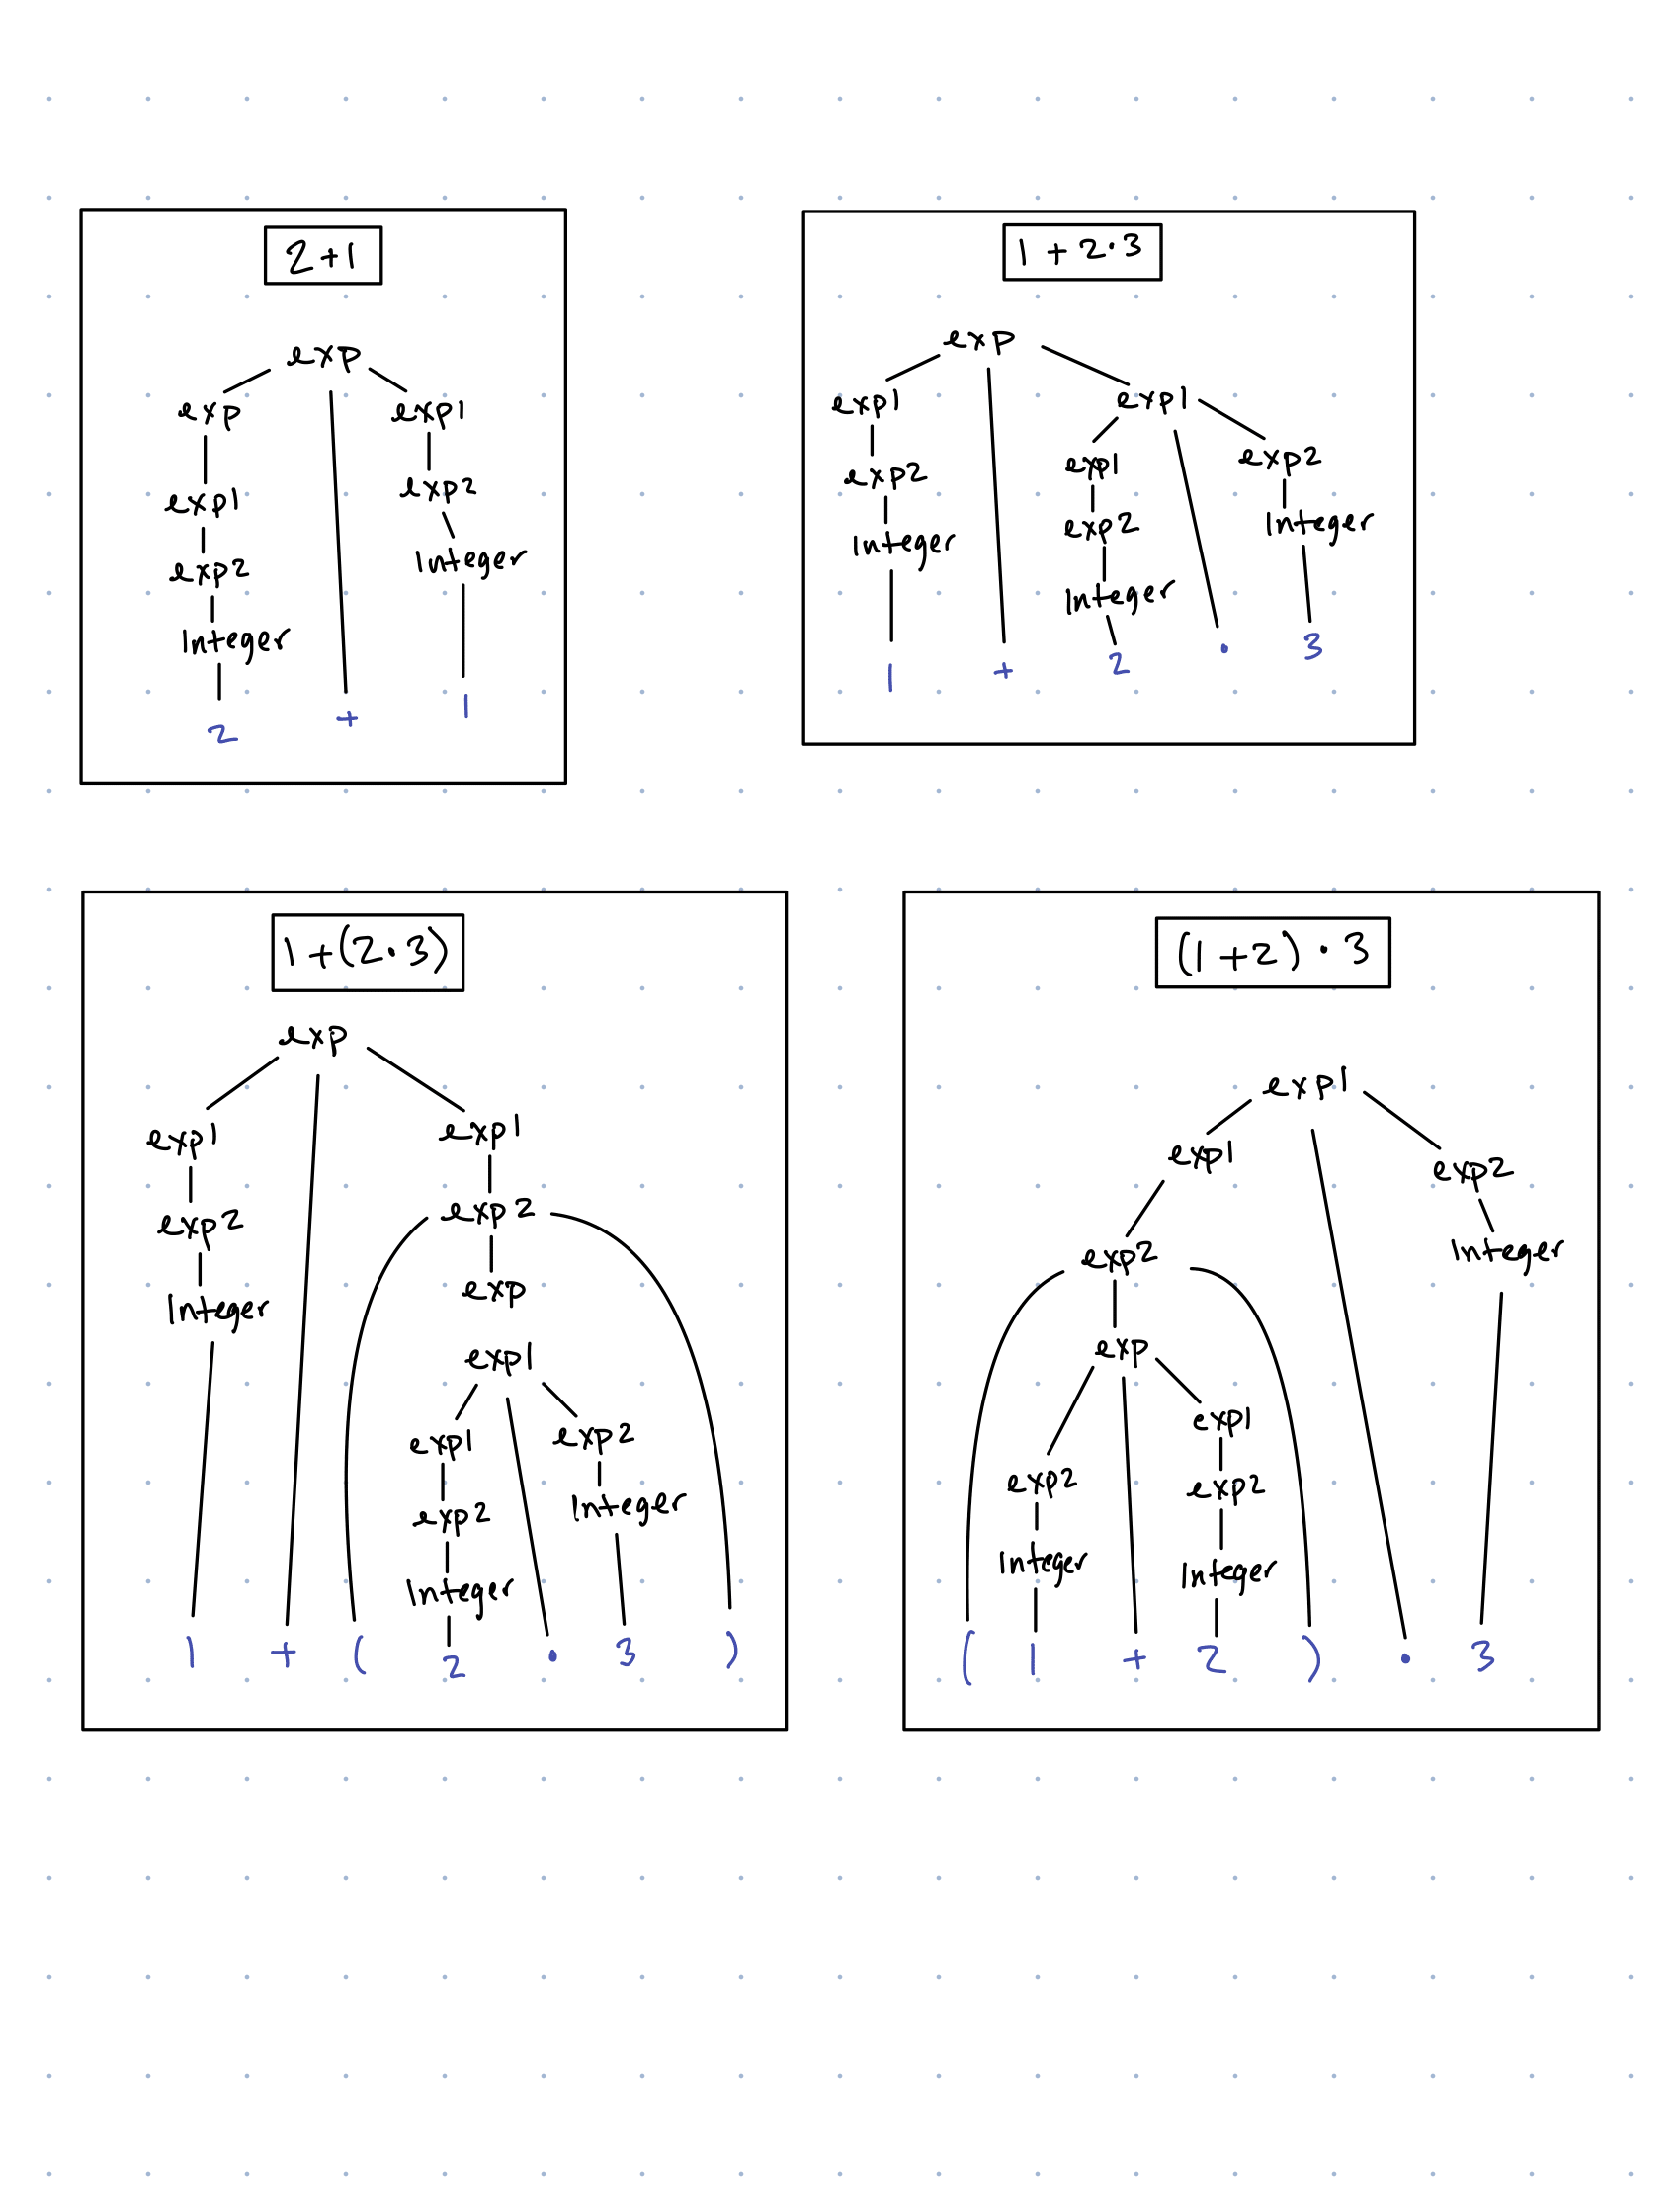
\includegraphics[scale=.5]{CPSC354 HW4-1.png}
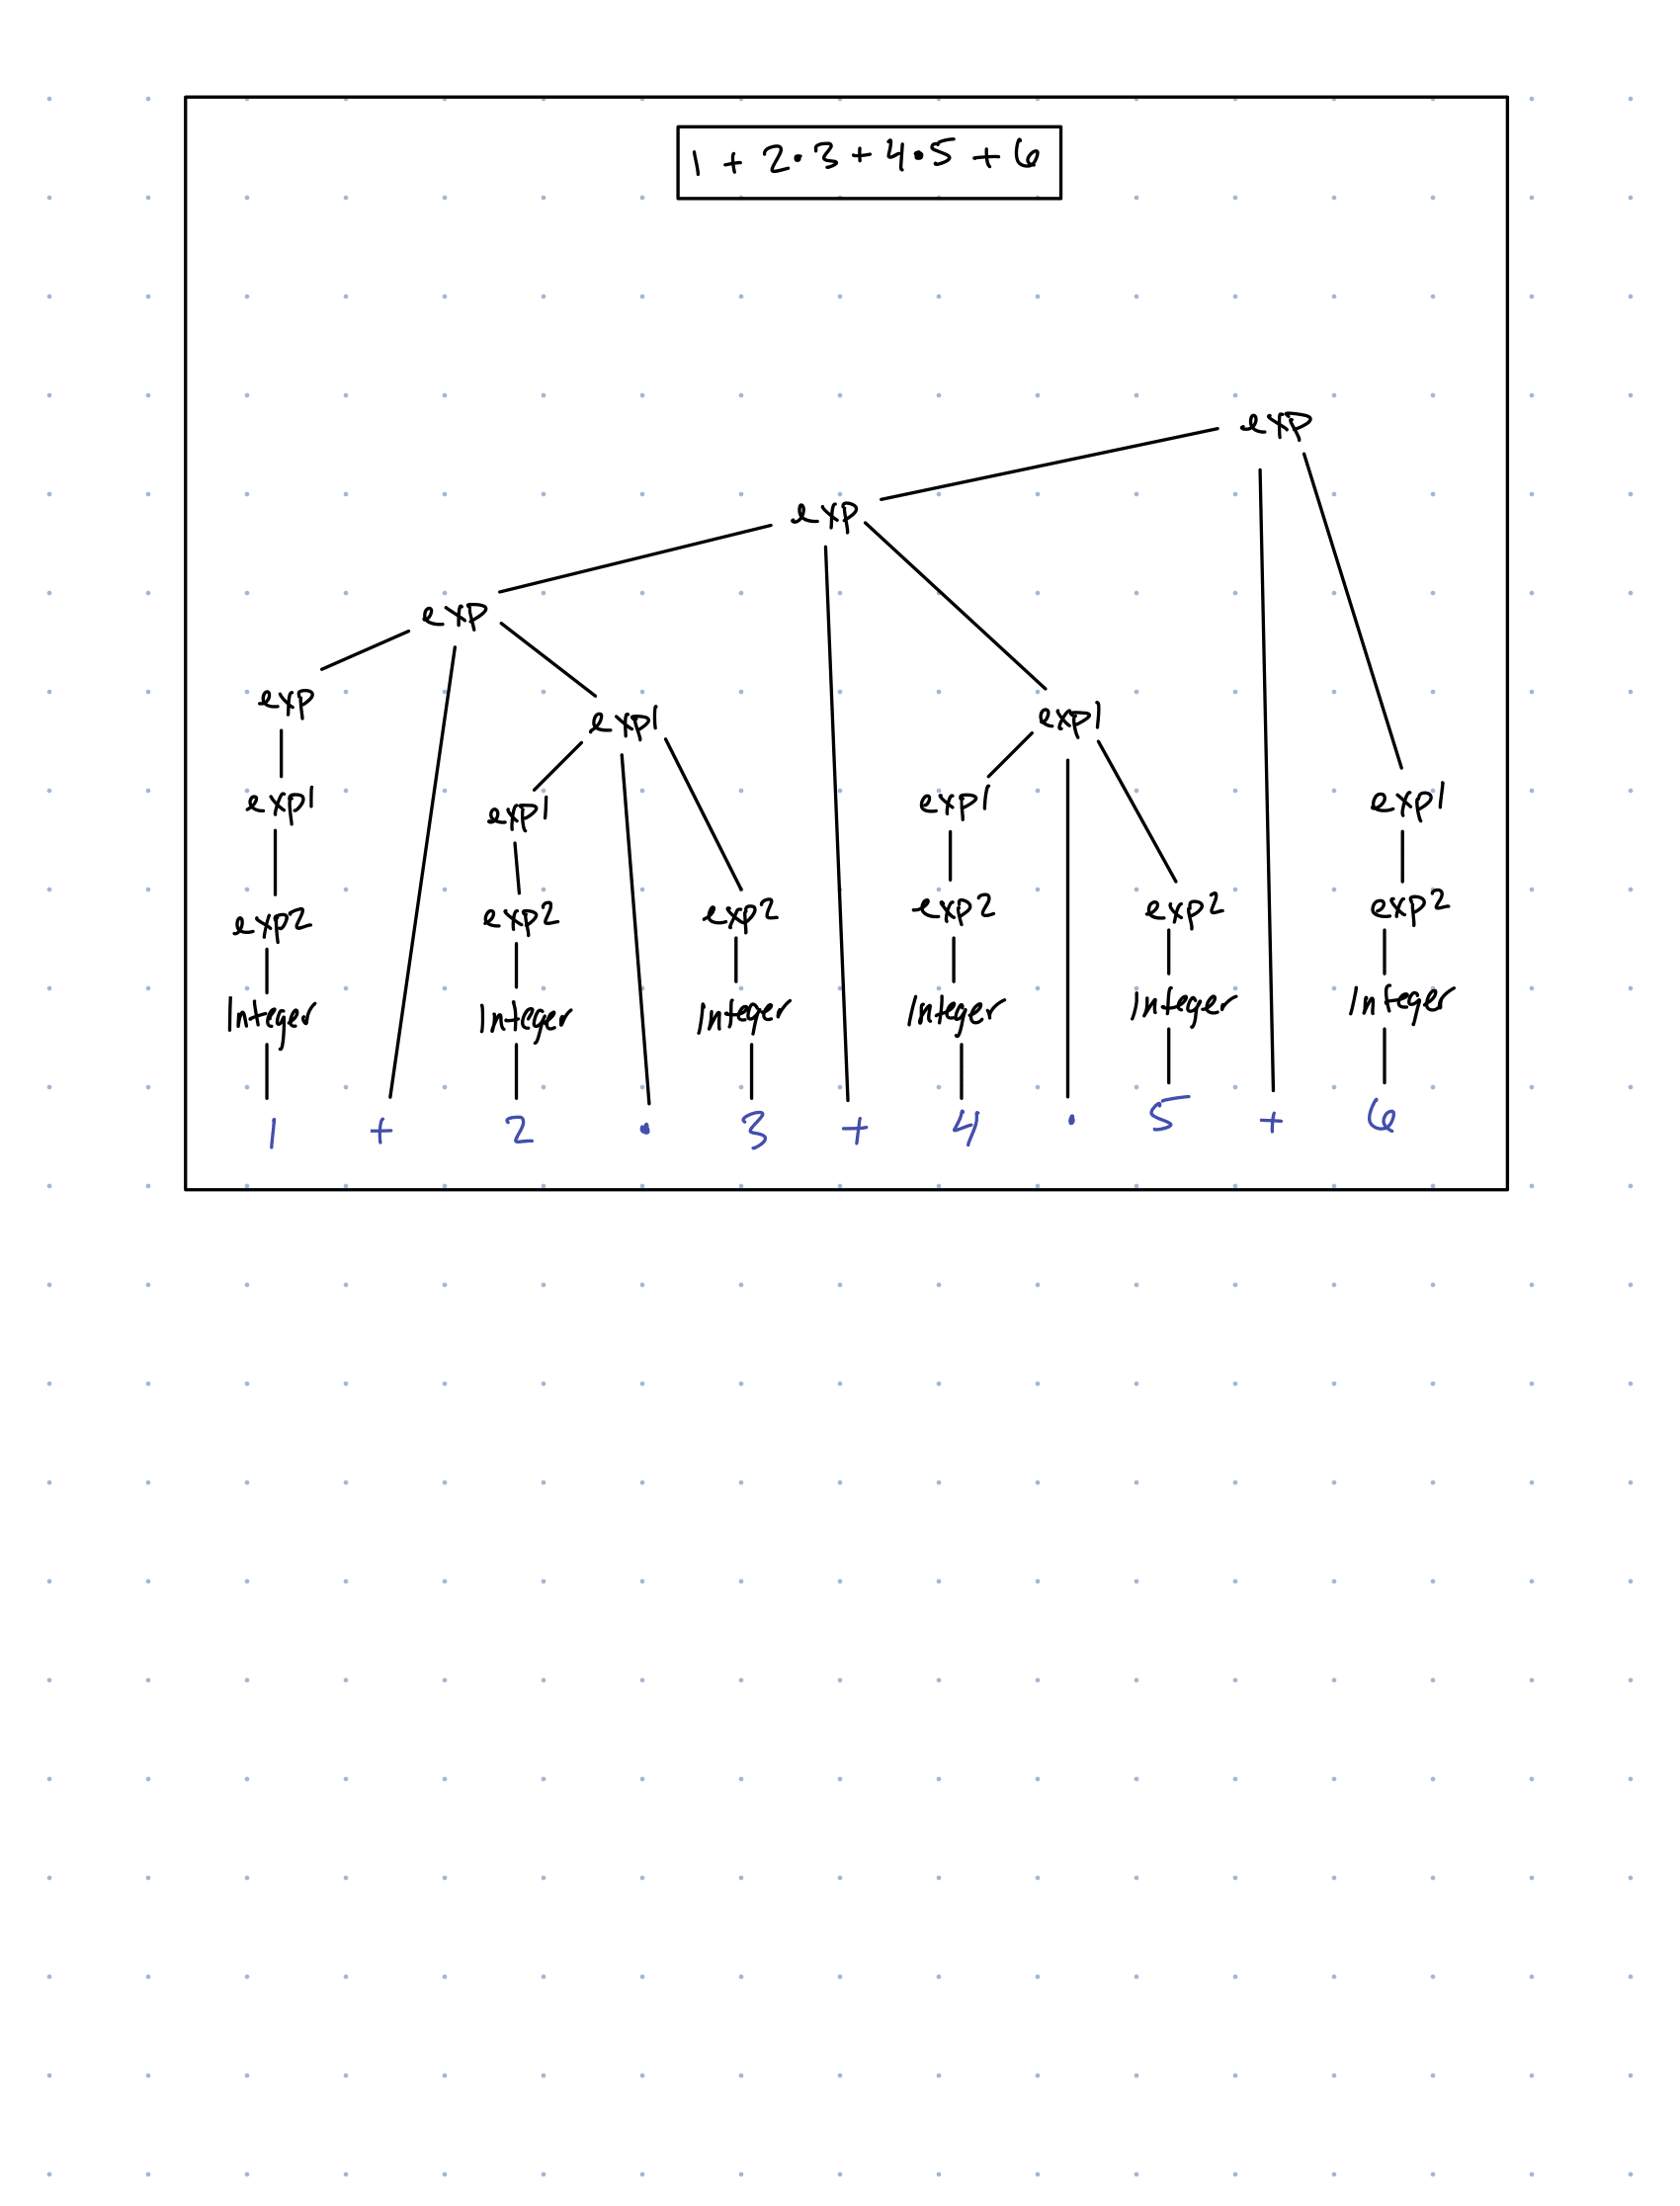
\includegraphics[scale=.6]{CPSC354 HW4-2.png}
\end{center}

\subsection{Week 4}

\subsubsection*{Notes} This week we discussed creating a calculator with CFGs and then about the next Lean world on logic. The logic world, similar to the math world, is about breaking down larger problems into manageable parts and tackling them one by one. If we can prove every infitessimal aspect of a larger problem, then we solve that large problem. I have really enjoyed working in the logic world so far because it is very similar to code design in game development. In game development, there are a number of components that control more context specific components, from the most high-level management context to the most basic mechanic. 

\subsubsection*{Question} Similar to Lianal's question, why does the logic world in Lean allow for varying syntax, while the math Lean world did not? Is this reflected in real (written) math/logic proofs?

\subsubsection*{Homework}

\subsubsection*{Level 1 - Exactly! It's in the premise}
Assumptions: $(P : Prop)(todo\_list : P) : P := by$

\[
\begin{aligned}
  (1)&\text{ exact todo\_list}
\end{aligned}
\]

\subsubsection*{Level 2 - And Introduction}
Assumptions: $(P S : Prop)(p: P)(s : S) : P \wedge S := by$

\[
\begin{aligned}
  (1)&\text{ exact ⟨ p, s ⟩}
\end{aligned}
\]

\subsubsection*{Level 3 - The Have Tactic}
Assumptions: $(A I O U : Prop)(a : A)(i : I)(o : O)(u : U) : (A \wedge I) \wedge O \wedge U := by$

\[
\begin{aligned}
  (1)& \text{ have ai } \text{:= and\_intro a i}\\
  (2)& \text{ have ou } \text{:= and\_intro o u}\\
  (3)& \text{ exact ⟨ ai, ou ⟩}
\end{aligned}
\]

\subsubsection*{Level 4 - And Elimination}
Assumptions: $(P S : Prop)(vm: P \wedge S) : P := by$

\[
\begin{aligned}
  (1)& \text{ have p } \text{:= vm.left}\\
  (2)& \text{ exact p}
\end{aligned}
\]

\subsubsection*{Level 5 - And Elimination 2}
Assumptions: $(P Q : Prop)(h: P \wedge Q) : Q := by$

\[
\begin{aligned}
  (1)& \text{ have q } \text{:= h.right}\\
  (2)& \text{ exact q}
\end{aligned}
\]

\subsubsection*{Level 6 - Mix and Match}
Assumptions: $(A I O U : Prop)(h1 : A \wedge I)(h2 : O \wedge U) : A \wedge U := by$

\[
\begin{aligned}
  (1)& \text{ exact ⟨ h1.left, h2.right ⟩ }
\end{aligned}
\]

\subsubsection*{Level 7 - More Elimination}
Assumptions: $(C L : Prop)(h: (L \wedge (((L \wedge C) \wedge L) \wedge L \wedge L \wedge L)) \wedge (L \wedge L) \wedge L) : C := by$

\[
\begin{aligned}
  (1)& \text{ exact h.left.right.left.left.right }
\end{aligned}
\]

\subsubsection*{Level 8 - Rearranging Boxes}
Assumptions: $(A C I O P S U : Prop)(h: ((P \wedge S) \wedge A) \wedge \neg I \wedge (C \wedge ¬O) \wedge ¬U) : A \wedge C \wedge P \wedge S := by$

\[
\begin{aligned}
  (1)& \text{ have c } \text{:= h.right.right.left.left}&\\
  (2)& \text{ have psa } \text{:= h.left}&\\
  (3)& \text{ have p } \text{:= psa.left.left}&\\
  (4)& \text{ have s } \text{:= psa.left.right}&\\
  (5)& \text{ have a } \text{:= psa.right}&\\
  (6)& \text{ exact ⟨ a, c, p, s ⟩ }
\end{aligned}
\]

\subsection{Week 5}

\subsubsection*{Notes} This week we discussed lambda higher order functions 
in the context of Lambda functions and had an interesting discussion about Curry 
Howard correspondance (currying) and languages. Lambda calculus functions are nameless, 
type-free functions. Within the context of lean, at least, this has been a difficult concept 
to grasp, because it is antithetical to the programming philosophy I have learned and practiced. 
However, the nature of lambda calculus is the same, but instead of relying on type-specific context, 
it relies on underlying logic within implicic type-deriving and preservation. I think this was 
confusing to me also because it throws explicit type safety out the window. On Thursday we discussed 
currying, $\alpha$-Conversion, $\beta$-Reduction, (and more) and had an interesting discussion about languages, 
and meaning behind language.  

\subsubsection*{Question} How do modern programming languages utilize (or avoid) lambda calculus in their syntax? In C\#, linq utilizes higher order functions encapsulating (what appears to be) explicitly defined lambda calculus functions, for example "enum.Where(x $\Rightarrow$ x.a $>$ 10)". It also seems like SQL syntax follows currying of lambda calculus functions, for example "SELECT * FROM \_ WHERE \_ ORDER BY \_", despite SQL not being a functional programming language.

\subsubsection*{Homework}

\subsubsection*{Level 1 - Cake Delivery Service}
Assumptions: $(P C: Prop)(p: P)(bakery\_service : P \rightarrow C) : C := by$

\[
\begin{aligned}
  (1)&\text{ exact (bakery\_service p)}
\end{aligned}
\]

\subsubsection*{Level 2 - Identity}
Assumptions: $(C: Prop) : C \rightarrow C := by$

\[
\begin{aligned}
  (1)& \text{ exact } \lambda \text{ var } \mapsto \text{ var }
\end{aligned}
\]

\subsubsection*{Level 3 - Cake Form Swap}
Assumptions: $(I S: Prop) : I \wedge S \rightarrow S \wedge I := by$

\[
\begin{aligned}
  (1)& \text{ exact } \lambda \text{ h : I } \wedge \text{ S } \mapsto \text{ and\_intro h.right h.left }
\end{aligned}
\]

\subsubsection*{Level 4 - And Elimination}
Assumptions: $(C A S: Prop) (h1 : C \rightarrow A) (h2 : A \rightarrow S) : C \rightarrow S := by$

\[
\begin{aligned}
  (1)& \text{ exact } \lambda \text{ c } \mapsto \text{ h2 (h1 c) }
\end{aligned}
\]

\subsubsection*{Level 5 - Riffin Snacks}
Assumptions: $(P Q R S T U: Prop) (p : P) (h1 : P \rightarrow Q) (h2 : Q \rightarrow R) (h3 : Q \rightarrow T) (h4 : S \rightarrow T) (h5 : T \rightarrow U) : U := by$

\[
\begin{aligned}
  (1)& \text{exact h5 (h3 (h1 p))}
\end{aligned}
\]

\subsubsection*{Level 6 - and\_imp}
Assumptions: $(C D S: Prop) (h : C \wedge D \rightarrow S) : C \rightarrow D \rightarrow S := by$

\[
\begin{aligned}
  (1)& \text{ exact } \lambda \text{ c d } \mapsto \text{ h (and\_intro c d) }
\end{aligned}
\]

\subsubsection*{Level 7 - and\_imp 2}
Assumptions: $(C D S: Prop) (h : C \rightarrow D \rightarrow S) : C \wedge D \rightarrow S := by$

\[
\begin{aligned}
  (1)& \text{ exact } \lambda \text{ ⟨c, d⟩ } \mapsto \text{ h c d }
\end{aligned}
\]

\subsubsection*{Level 8 - Distribute}
Assumptions: $(C D S : Prop) (h : (S \rightarrow C) \wedge (S \rightarrow D)) : S \rightarrow C \wedge D := by$

\[
\begin{aligned}
  (1)& \text{ have ⟨l, r⟩ := h}\\
  (2)& \text{ exact } \lambda \text{ s } \mapsto \text{ ⟨l s, r s⟩ }
\end{aligned}
\]

\subsubsection*{Level 9 - Uncertain Snacks}
Assumptions: $(R S : Prop) : R \rightarrow (S \rightarrow R) \wedge (\neg S \rightarrow R) := by$

\[
\begin{aligned}
  (1)& \text{ exact } \lambda \text{ r } \mapsto \text{ and\_intro ( } \lambda \text{ \_ } \mapsto \text{ r ) } \lambda \text{ \_ } \mapsto \text{ r}
\end{aligned}
\]

\subsection{Week 6}

\subsubsection*{Notes} This week we dove into theory discussions and lectures on application of currying, more complex lambda calculus and church numerals. To be honest, it is hard to remember much notes-wise because the theory was so intense, but I can say with confidence that I was confused - and embraced it! To help with my understanding, I looked for resources online and found this paper by Helmut Brandl titled \textbf{Limits of Computability in Lambda Calculus} (\url{https://hbr.github.io/Lambda-Calculus/computability/text.html}) which actually covered nicely what we have been learning about recently. In the preamble, Kurt Goedel's \textit{Godel Numbering} is discussed, and I thought the paper gave some interesting historical context to a memorable moment in logic and maths history; "In his famous incompleteness theorem (1931) Goedel demonstrated that paradoxical statements can be injected into all formalisms which are powerful enough to express basic arithmetics." Anyway, I digress. 

\subsubsection*{Question} Since lambda calculus is comprised of only abstraction and application, and cannot examine itself, how can infinitely recursing expressions like $(\lambda x.xx)(\lambda x.xx)$ terminate, and is that simply a non-issue? On a computer this would cause a stack overflow, but conceptually it follows the rules. Aside from physical computational constraints, are there other factors that do not permit translation from lambda calculus theory to implementation?

\subsubsection*{Homework}

1) Reduce the following lambda term:\\
\[
\begin{aligned}
  & \text{  ((\textbackslash m.\textbackslash n. m n) (\textbackslash f.\textbackslash x. f (f x))) }\\
  & \text{  (\textbackslash f.\textbackslash x. f (f (f x))) }\\
  \\
  (1)& \text{   ((\textbackslash m.\textbackslash n. m n) (\textbackslash f.\textbackslash x. f (f x))) (\textbackslash f2.\textbackslash x2. f2 (f2 (f2 x2)))}\\
  \\
  (2)& \text{   (\textbackslash n. (\textbackslash f.\textbackslash x. f (f x)) n) (\textbackslash f2.\textbackslash x2. f2 (f2 (f2 x2)))}\\
  \\
  (3)& \text{   (\textbackslash f.\textbackslash x. f (f x)) (\textbackslash f2.\textbackslash x2. f2 (f2 (f2 x2)))}\\
  \\
  (4)& \text{   \textbackslash x. (\textbackslash f2.\textbackslash x2. f2 (f2 (f2 x2))) ((\textbackslash f2.\textbackslash x2. f2 (f2 (f2 x2))) x)}\\
  \\
  (5)& \text{   \textbackslash x.(\textbackslash f2.\textbackslash x2. f2 (f2 (f2 x2))) (\textbackslash x2. x (x (x x2)))}\\
  \\
  (6)& \text{   \textbackslash x.\textbackslash x2.(\textbackslash x2. x (x (x x2))) ((\textbackslash x2. x (x (x x2))) ((\textbackslash x2. x (x (x x2))) x2))}\\
  \\
  (7)& \text{   x\textbackslash .\textbackslash x2.(\textbackslash x2. x (x (x x2))) ((\textbackslash x2. x (x (x x2))) (x (x (x x2))))}\\
  \\
  (8)& \text{   x\textbackslash .\textbackslash x2.(\textbackslash x2. x (x (x x2))) (x (x (x (x (x (x x2))))))}\\
  \\
  (9)& \text{   \textbackslash x.\textbackslash x2.x (x (x (x (x (x (x (x (x x2))))))))}\\
\end{aligned}
\]

2) Explain what function on natural numbers $(\backslash m. \backslash n. m n)$ implements:\\
\\This lambda expression implements similar behaviour to the identity function, but with church numerals. It returns the application of $m$ on $n$.

\subsection{Week 7}

\subsubsection*{Notes} This week we started working on assignment 3, which is creating an interpreter of lambda calculus. We started with a base interpreter that does not perform as expected in all cases. Uses this as a template, we started working to understand its limitations and to address them. Dr. Kurz gave a brief overview of using the debugger in VScode, which will be a valuable asset during the development of the interpreter. 

\subsubsection*{Question} I recently learned about programming language where the language aspect is built upon the Figma whiteboard feature. See \url{https://devpost.com/software/unreal-engjam} (Thanks @JadenJ for sharing!). The language was developed in TypeScript and generates an AST. I was intrigued into what other mediums can serve as effective interfaces; node-based visual scripting (e.g. Unity, UE) is an immediate thought. What other human $\rightarrow$ code interfaces exist? What makes a medium an effective tool for interfacing with code?

\subsubsection*{Homework}

Homework this week is working on assignment 3.

\subsection{Week 8}

\subsubsection*{Notes} This week in class we worked on Assignment 3 and talked about strategies for reducing lambda expressions. With the goal of reducing lambda expressions to normal form we learned and practiced using the VSCode debugger to navigate the interpreter program.

\subsubsection*{Question} 

\subsubsection*{Homework}
Please see \textbf{Homework} under \textbf{Week 9} below for the combined homework for weeks 8 and 9.

\subsection{Week 9} 

\subsubsection*{Notes} This week we worked on assignment 3 in class and talked more about the logic behind reducing lambda expressions.

\subsubsection*{Question} What separates the possible use cases of call-by-name and call-by-value methodologies? For example, I would think that a type-safe environment would prefer call-by-value because the input variable is evaluated before substitution takes place. 

\subsubsection*{Homework}
Please see \url{https://github.com/szykozlowski/lambda-calc-assignment/blob/main/WritttenQuestions.md} for our team's answers to this week's homework questions.


\subsection{Week 10}

\subsubsection*{Notes} This week in class we talked about algorithms as rewriting systems, the characteristics these expressions involving confluence, termination, and unique normal forms. We went into detail talking about the buggle sort as an example of an ARS. 

\subsubsection*{Question} In the notes, an ARS is described as a non-deterministic algorithm for determining equivalency within the ARS. What about ARSs makes this process non-deterministic, and how can a non-deterministic process define equivalency?

\subsubsection*{Homework}

\subsection{Week 11}

\subsubsection*{Notes} On tuesday we played around with the sliding puzzle and discussed solvability and invariability. Invariability is a system that doesn't change when transformations are applied to it.

\subsubsection*{Question} 

\subsubsection*{Homework}

\[
\begin{aligned}
  (1)& \textbf{ What did you find most challenging when working through Homework 8/9 and Assignment 3?}\\
     &  \text{The most challenging aspect was trying to figure out what functionality the program lacked. Because the}\\ 
     &  \text{program is recursive, tracking the steps individually was difficult.}\\
     &\\
  (2)& \textbf{ How did you come up with the key insight for Assignment 3?}\\
     &  \text{We came up with the key insight into solving assignment 3 by focusing less on the the program and more}\\
     &  \text{on what, conceptually, needed to happen at each iteration of the evaluation process. This way, we could}\\
     &  \text{see that any lam statement in the AST needed to be preceeded by an app statement, and figure out }\\
     &  \text{exactly which step was being missed by the program.}\\
     &\\
  (3)& \textbf{ What is the most interesting takeaway from Homework 8/9 and Assignment 3?}\\
     &  \text{My most interesting takeaway definitely concerned the debugger. Conceptually learning more abot how an}\\
     &  \text{interpeter program works and recurses was exciting, but learning about another tool and getting it}\\
     &  \text{under my belt felt very valuable.}\\
\end{aligned}
\]

\subsection{Week 11}

\subsubsection*{Notes} On Tuesday we walked through an example of an ARS that described XOR behaviour. We applied the relationship between the ARS and the XOR truth table to an even/odd table, as well. This helped me to think about ARS's as describing non-determinate systems, because the behaviour that they describe (the equivalency behaviour) can be applied to many contexts, in the same way that a function doesn't care about the context that it is called from, or the context of its parameters. We continued to work on understanding other examples of ARSs. 

\subsubsection*{Question} When thinking about how an ARS could describe a physiological system (e.g. homeostasis), is it possible to construct an ARS that can adapt its ruleset over time? For example, the characteristic of homeostasis, or rather its impact on bodily systems, is different if the person is in very cold weather as opposed to very hot weather.

\subsubsection*{Homework}

\begin{center}
  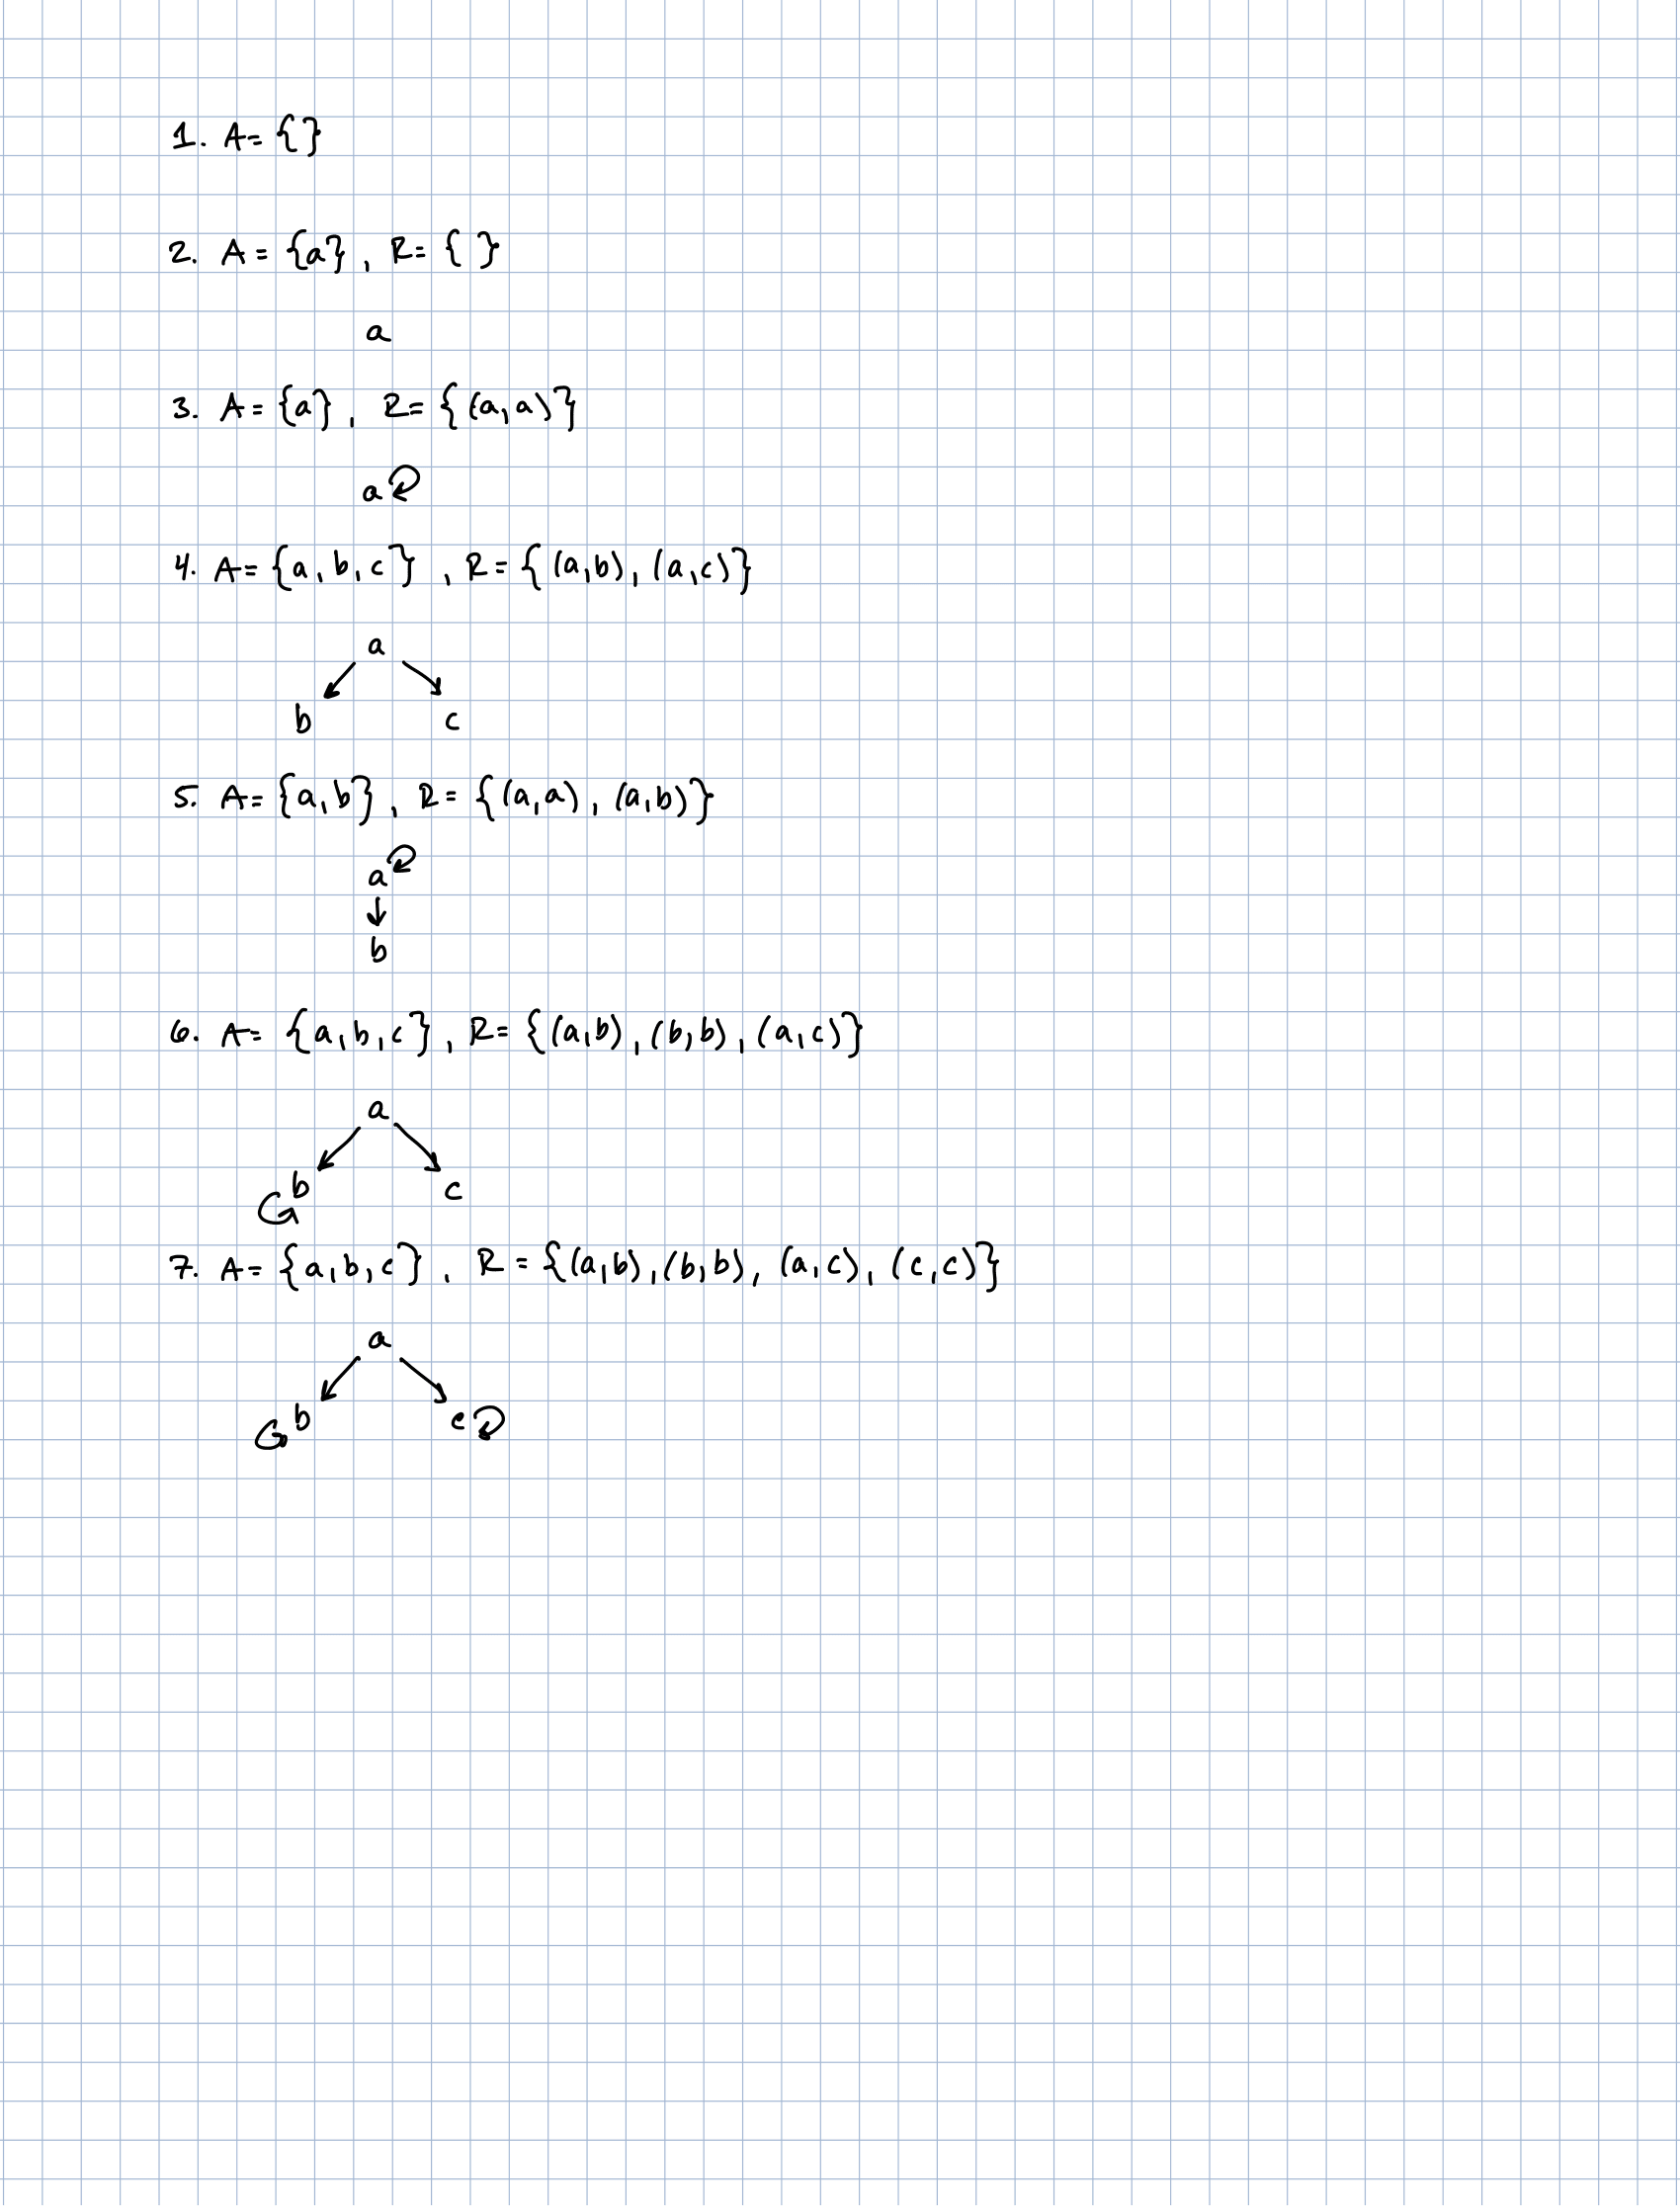
\includegraphics[scale=.75]{CPSC354 HW11-1.png}\\
  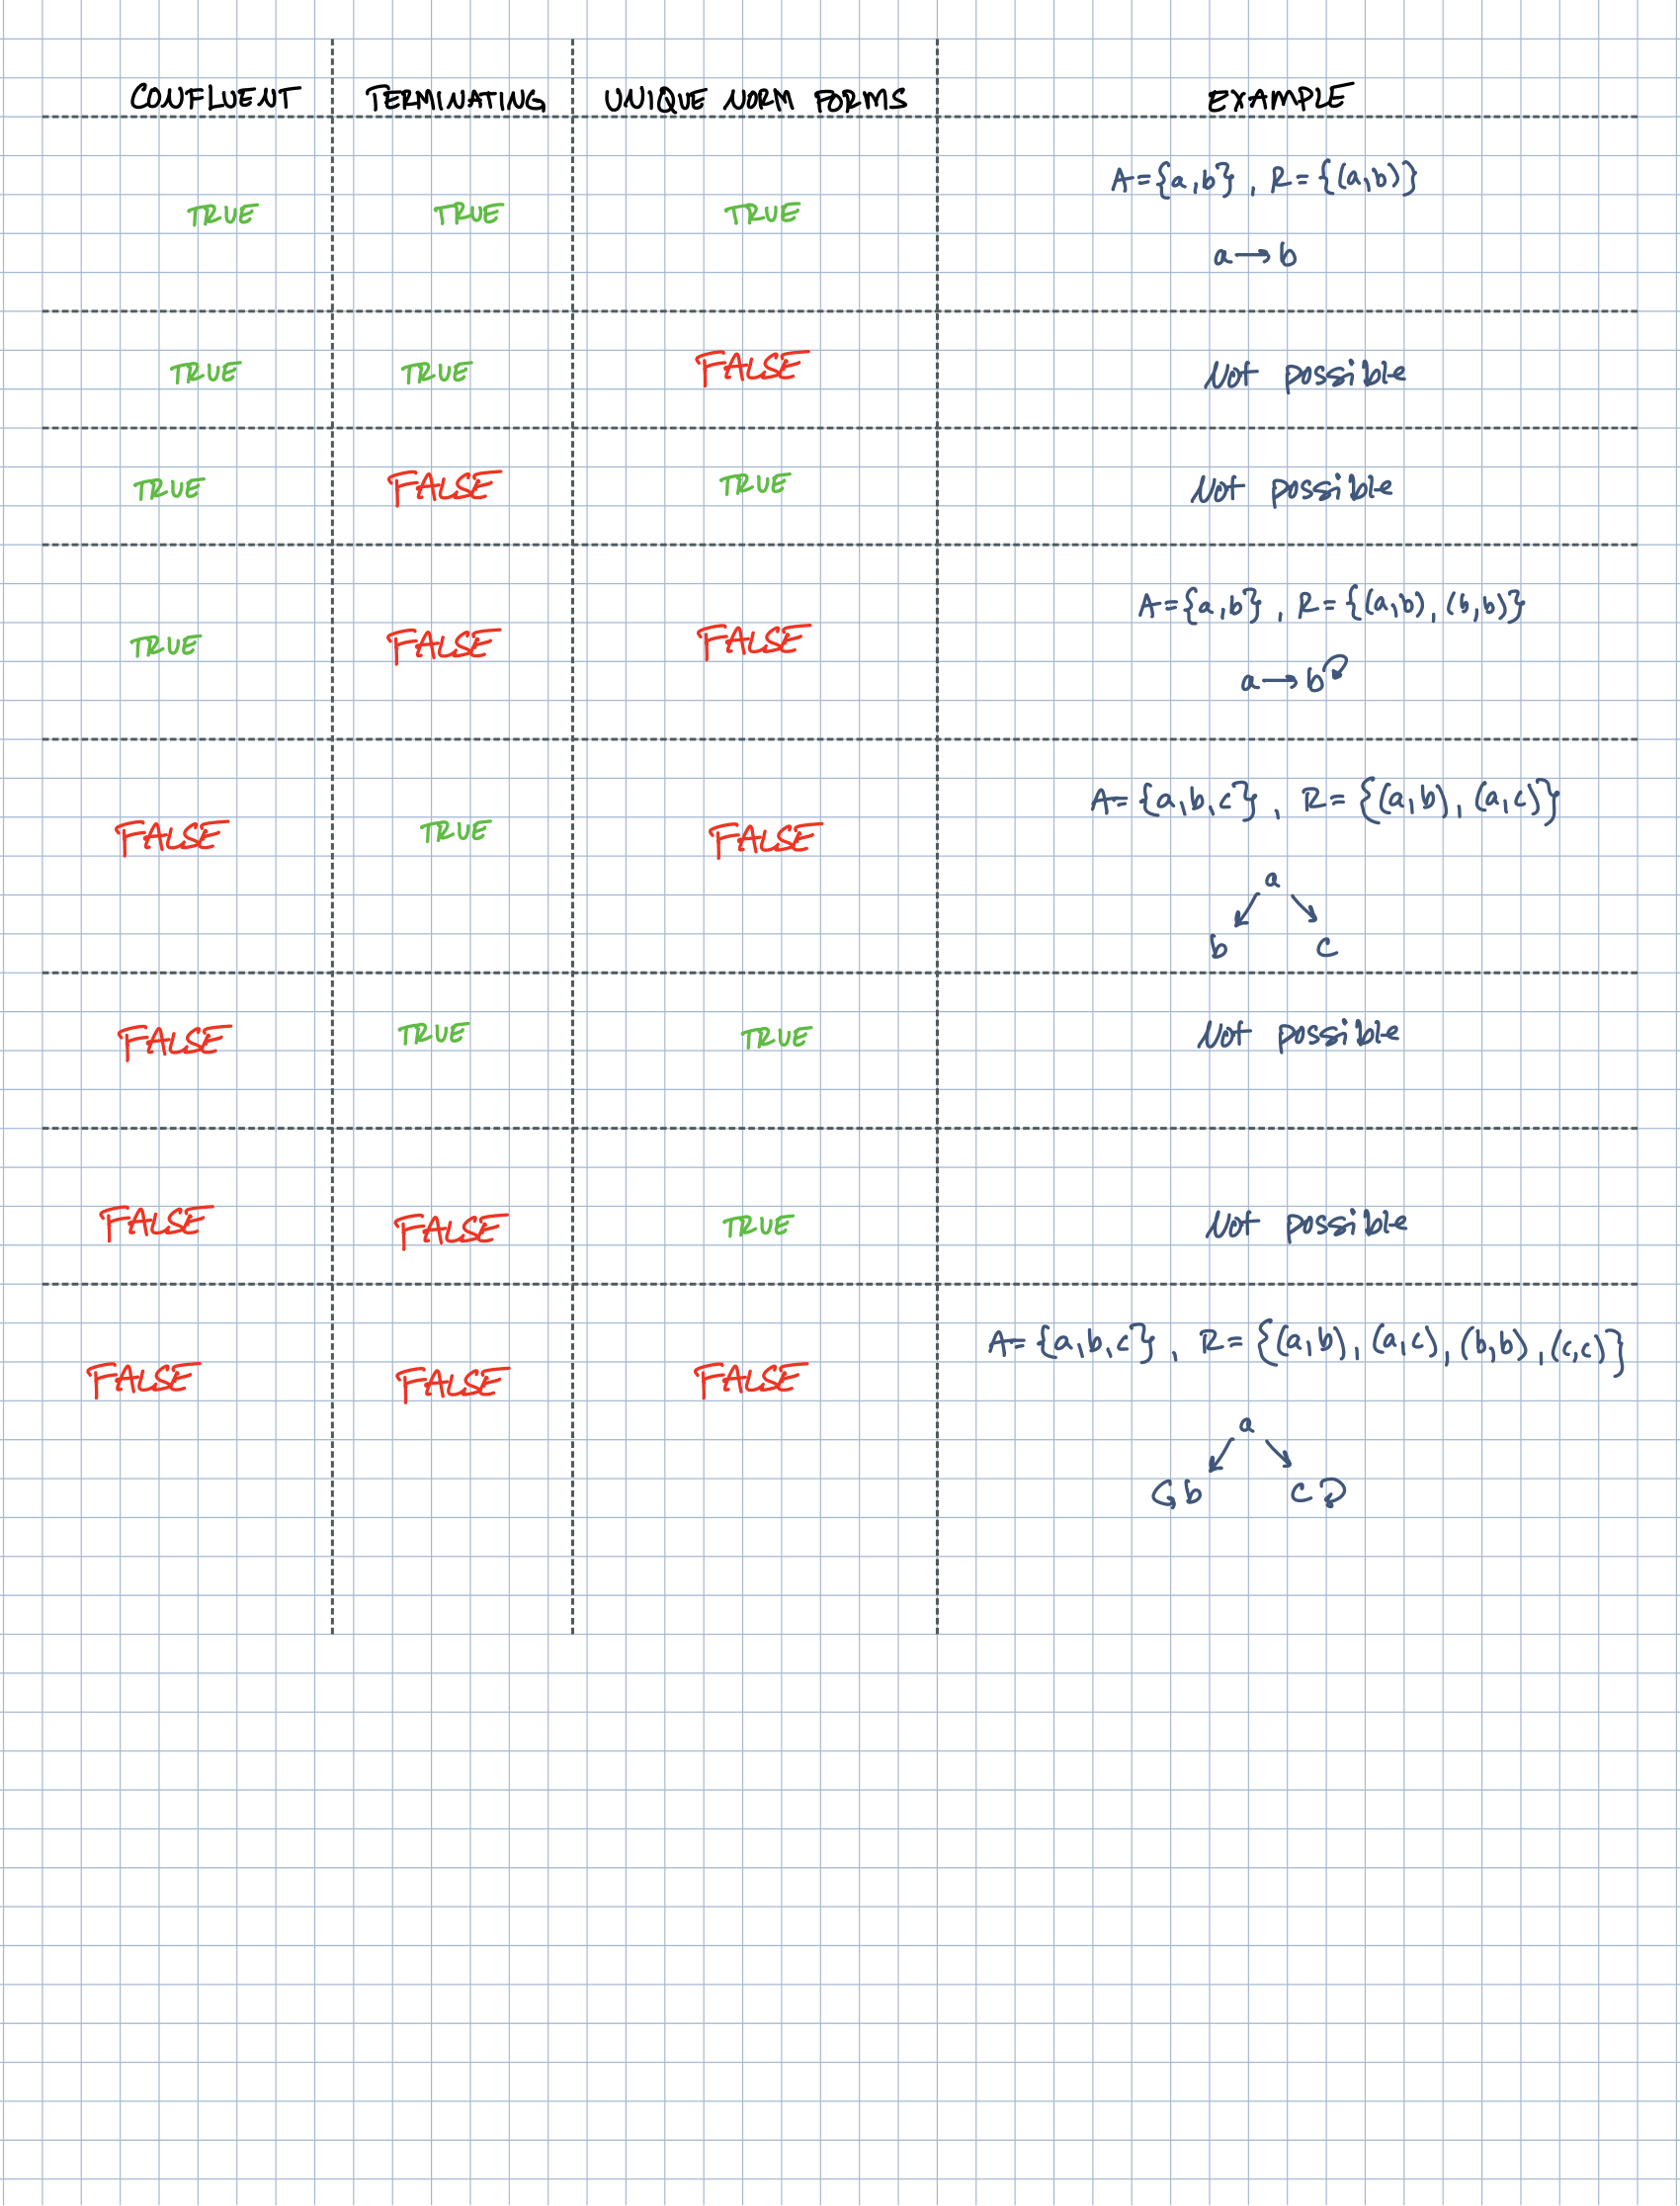
\includegraphics[scale=.75]{CPSC354 HW11-2.png}
  \end{center}

\subsection{Week 12}

\subsubsection*{Notes} This week in class we talked about invariants, specifically within the context of a sliding puzzle on Tuesday. This puzzle was an interesting demonstration of how moving pieces around a puzzle which was impossible to begin with will never make it solvable, and vice versa. This also leads off of the discussion that we had about splitting computations into different equivalence classes, such that the defining characteristics of those computations will always remain regardless of how the system is changed. We discussed fixed-point combinators on Thursday, and how they can be used to implement recursion into lambda calculus. To do this we re-visited conditionals in lambda calculus and defined naming.

\subsubsection*{Question} Are there other methods of performing recursion in lambda calculus besides fixed-point combinators? Does the definition of naming functional or is it just syntactic sugar?

\subsubsection*{Homework}

\[
\begin{aligned}
  \text{ let fact(3)} &\equiv  \text{ ( fix (f.x x)) in 3} &\dashleftarrow\text{def of let rec}\\
  &\equiv\beta\text{ f.x ( fix (f.x x)) in 3} &\dashleftarrow\text{beta rule: sub fix F}\\
  &\equiv\beta\text{ 3 * ( fix (f.x x)) in 2} &\dashleftarrow\text{beta rule: sub fix F}\\
\end{aligned}
\]

\section{Lessons from the Assignments}

(Delete and Replace): Write three pages about your individual contributions to the project.

On 3 pages you describe lessons you learned from the project. Be as technical and detailed as possible. Particularly valuable are \emph{interesting} examples where you connect concrete technical details with \emph{interesting} general observations or where the theory discussed in the lectures helped with the design or implementation of the project.

Write this section during the semester. This is approximately a quarter of apage per week and the material should come from the work you do anyway. Just keep your eyes open for interesting lessons.

Make sure that you use \LaTeX{} to structure your writing (eg by using subsections).

\section{Conclusion}\label{conclusion}

(Delete and Replace): (approx 400 words) A critical reflection on the content of the course. Step back from the technical details. How does the course fit into the wider world of software engineering? What did you find most interesting or useful? What improvements would you suggest?

\begin{thebibliography}{99}
\bibitem[BLA]{bla} Author, \href{https://en.wikipedia.org/wiki/LaTeX}{Title}, Publisher, Year.
\end{thebibliography}

\end{document}
